\chapter{Implementierung}\label{ch:implementation}



%Für unsere Implementation wird für das Zwischenspeichern von Daten ein Serviceworker eingesetzt. Serviceworker können wie ein Proxy zwischen dem Webbrowser und dem Webserver agieren, welcher die Webseite bereitstellt. Stellt ein Browser eine Anfrage, so wird diese vom Serviceworker abgefangen. Der Serviceworker schaut zunächst in seinem Cache, der sog. IndexDB, ob er die gestellte Anfrage beantworten kann. Ist dies nicht der Fall, so wird die Anfrage an den Webserver weitergeleitet. Wird die gleiche Anfrage nochmals gestellt, kann diese aus dem Cache beantwortet werden, da gestellte Anfragen eine gewisse Zeit lang zwischengespeichert werden.
%\begin{figure}[!h]
%	\centering
%	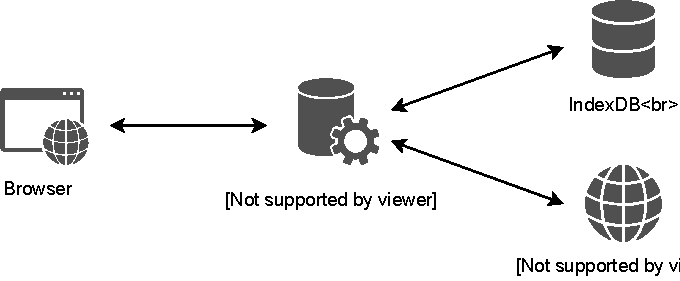
\includegraphics[width=0.8\textwidth]{figures/ServiceWorker}
%	\caption[A Figure Short-Title]{A Figure Title}
%	\label{fig:sequenceDiagram}
%\end{figure}
%
%
%Die von uns eingesetzte Technologie zur Übertragung von Daten zwischen Browsern ist WebRTC. WebRTC ist ein offener Standard und ermöglicht es Browser paarweise zwecks Datenaustausch zu verbinden. Der große Vorteil dieser Technologie ist, dass sie direkt von modernen Browsern unterstützt wird, wodurch keine zusätzliche Software installiert werden muss. Konkret wird von uns ein sog. DataChannel genutzt.
%
%Für den Datenaustausch müssen wechselseitig DataChannel zueinander aufgebaut werden. Die Ausgangslage ist, dass die Schüler wissen, dass es den anderen gibt, aber nicht wie der jeweils andere zu erreichen ist. Um diese Problematik zu lösen, existiert ein Vermittlungsserver (Signaling server).
%
%Als erstes werden Informationen, über die Verbindung die aufgebaut werden soll, an den Signaling server gesendet. Technisch wird ein SDP-offer gesendet, wobei SDP für Session Description Protocol steht. Dieses SDP-offer leitet der Signaling server an die Schüler in der Klasse/Schule weiter. Geantwortet wird mit einer SDP-answere, welche Informationen über die abgestimmte Verbindung enthält und über den Signaling server zurück geleitet wird.
%
%Damit eine direkte Verbindung aufgebaut werden kann, müssen über den Signaling server noch weitere Informationen wie ICE-Kandidaten ausgetauscht werden. ICE steht hierbei für Interactive Conectivity Establishment und ist fester Bestandteil von WebRTC. Es ist für den Aufbau der Browser-zu-Browser-Verbindung verantwortlich. ICE-Kandidaten enthalten hauptsächlich Informationen darüber wie ein bestimmter Nutzer erreichbar ist (also z.B. private oder öffentliche IP-Adresse). Ermittelt werden diese ICE-Kandidaten mithilfe eines STUN-Servers und dem dazugehörigen Session Traversal Utilities for NAT (STUN) Protokoll. Wie der Name des Protokolls schon verrät, wird es vor allem benötigt um auch Nutzer erreichen zu können die keine eigene öffentliche IP-Adresse besitzen, bei denen also Network address translation (NAT) eingesetzt wird. Dies ist aufgrund der mangelnden Anzahl an IPv4-Adressen bei fast jedem Internetnutzer der Fall.
%
%In dem Signaling server selbst wird die Logik abgebildet, wie die Klassen und Schüler miteinander in Verbindung stehen. Implementiert wurde dieser mit socket.io, da die native Klassenorganisation und Websocket-Technologie sich nahezu perfekt für unser Szenario anbot.

\section{Architectur}

\begin{itemize}
  \item Server architektur diagram --> Server, Stun, CDN, P2P CDN
  \item Plugin Architektur -->  
\end{itemize}

\begin{figure}[!h]
	\centering
	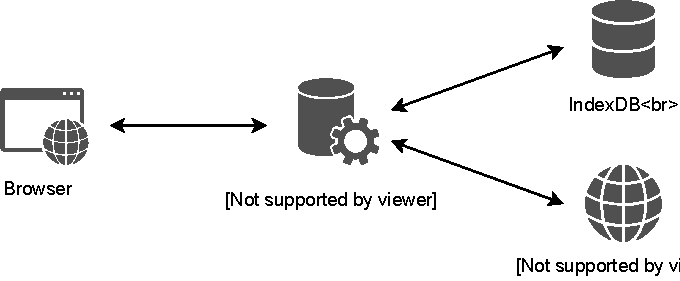
\includegraphics[width=0.8\textwidth]{figures/ServiceWorker}
	\caption[A Figure Short-Title]{A Figure Title}
	\label{fig:sequenceDiagram}
\end{figure}

\subsection{Service worker}
\begin{itemize}
  \item warten bis sw active ist/alle verbindungen ready sind vs request normal durchgehen lassen bis alles fertig ist.
  \item Requests werden erst nach erfolgreicher registrierung behandelt
  \item clients.claim + skip waiting für den ersten aufruf (12)
\end{itemize}


\subsection{Tests}

\begin{itemize}
  \item mocha
  \item chai
  \item karma
  \item event handler testen
  \item registrieren/abmelden --> test helper
\end{itemize}

%- mocha
%- chai
%- karma
% Event handler testen
% 	- registrieren/abmelden --> test helper

\section{Ressourcen Management}


\subsection{Update Protokoll}

\subsection{Quota limits}



\begin{itemize}
  \item benötigte speichermenge wird geschätzt
  \item headersize plus 'Content-Length' header wert
  \item solange löschen bis genug speicher frei ist
\end{itemize}

\section{Signaling Server}
The signaling server itself uses socket.io and can be found here. The client ID is created there and is essential for the lifecycle of a peer in the whole network. It is not clear if the client IDs given by socket.io always have the same length. Therefore, client IDs will be padded to a maximal length of 24. This is necessary because the client IDs need to be sent via the binary datachannel and consequently, this requires a fixed length.


\begin{itemize}
  \item websockets socket io
  \item gleicher data channel zur Bildung von meshs
\end{itemize}


\section{Message protocol}
%In unserer Implementation wird, sobald eine neuer Besucher der Webseite hinzukommt, sofort ein DataChannel, mittels WebRTC, STUN, ICE und Signaling server zu allen anderen aktiven Besuchern aufgebaut. Über diesen werden zu zwei Zeitpunkten Informationen darüber ausgetauscht, welche Ressourcen bei dem jeweiligen Nutzer vorliegen: Direkt nach Aufbau des DataChannels und immer dann, wenn ein Nutzer eine neue Ressource (aus dem Internet oder lokal) geladen und in seinem Cache gespeichert hat:

\begin{figure}[!h]
	\centering
	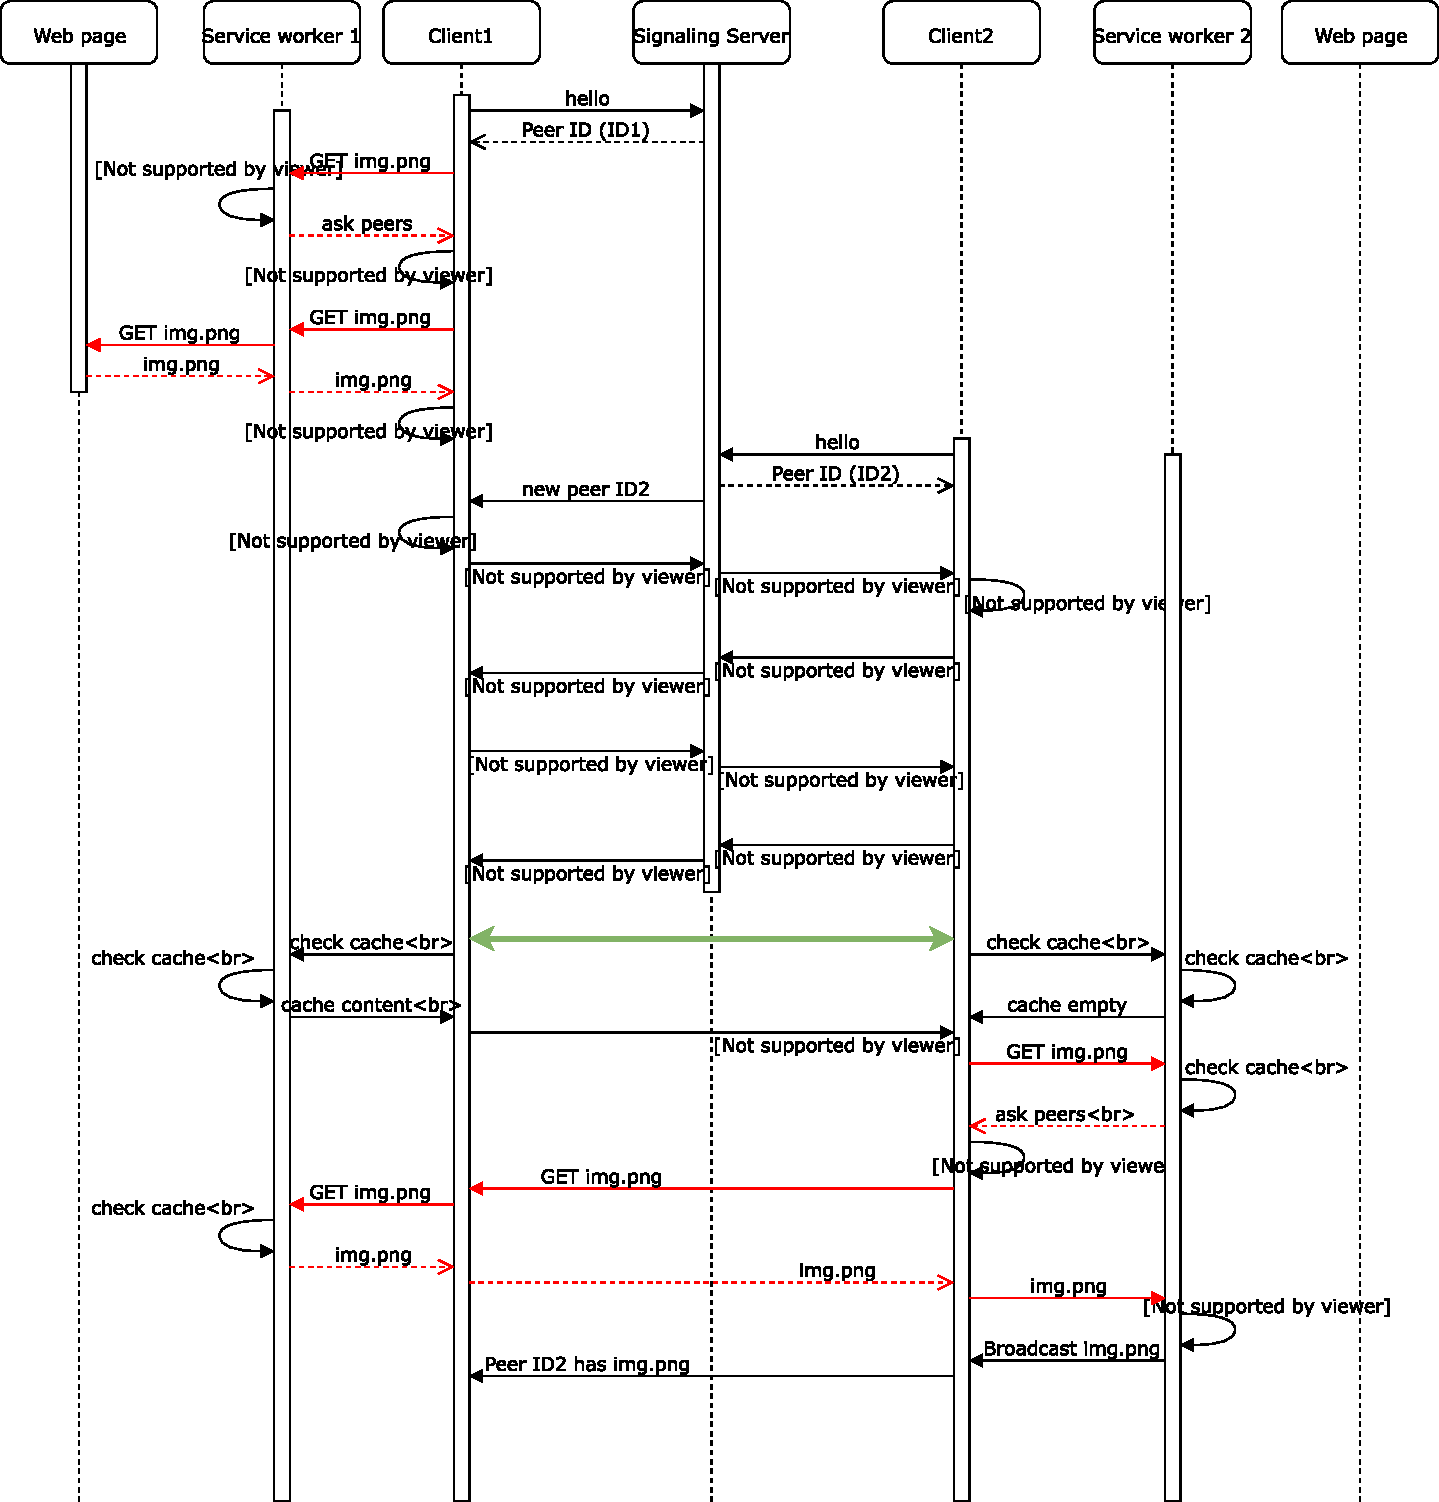
\includegraphics[width=0.8\textwidth]{figures/SequenceDiagram}
	\caption[A Figure Short-Title]{A Figure Title}
	\label{fig:sequenceDiagram}
\end{figure}

%Client 1 (C1) ist der erste der die Webseite aufruft. Er registriert sich beim Signaling server und fragt im Anschluss img.png an (rot). Da noch niemand anders auf der Seite ist von dem er die Ressource bekommen könnte und er zudem die Ressource nicht in seinem Cache hat, wird img.png über das Internet vom Webserver geladen. Client 2 (C2) ruft nun ebenfalls die Webseite auf und registriert sich beim Signaling server. Dieser benachrichtigt C1, dass ein neuer Teilnehmer registriert wurde, woraufhin C1 einen Verbindungsaufbau zu C2 einleitet. Steht die direkte Verbindung zwischen C1 und C2 (grün), teilt C1 C2 den Inhalt seines aktuellen Caches mit. Fragt C2 img.png an (rot), weiß er so, dass er diese von C1 anfragen kann. Hat er img.png erhalten, teilt er allen anderen Teilnehmern (in diesem Fall nur C1) mit, dass auch er jetzt img.png als Ressource in seinem Cache hat

\subsection{hash updates}
message types
\section{Data serialization}

\begin{itemize}
  \item SCTP(DataChannel) message size limit 16kiB
  \item chunking reassembling nötig
  \item Performance einbussen
  \item abToMessage und sendToPeer
\end{itemize}

% SCTP(DataChannel) message size limit 16kiB
% chunking reassembling nötig
% _abToMessage() und _sendToPeer
% Performance einbußen

%Currently, it is only possible to send messages not larger than 16kiB via the RTCDataChannel. In order to send larger messages chunking and reassembling is necessary. These procedures take place in the _abToMessage() and _sendToPeer() methods in the peer.js file.

\section{Mesh Zuordnung}
% data Channels zur mesh verbindung definiert über Anwendung
% ip subnetz erkennung wie implementiert?

\section{Reusability}

\section{System Test}

\section{Storage quotas}
navigator.storage.estimate()

The \textvtt{minted} package is really nice for code formatting.

\begin{listing}[h]
	\inputminted{ruby}{listings/context-data-transform.rb}
	\caption{Some Code Snipped}
	\label{lst:code-snipped}
\end{listing}

\section{Resource loading}
